\documentclass[11pt]{article}

\usepackage[margin=1in]{geometry}
\usepackage{setspace}
\onehalfspacing
\usepackage{graphicx}
\graphicspath{report_images/}
\usepackage{appendix}
\usepackage{listings}
\usepackage{float}
\usepackage{multirow}
\usepackage{amsthm}
% The next three lines make the table and figure numbers also include section number
\usepackage{chngcntr}
\counterwithin{table}{section}
\counterwithin{figure}{section}
% Needed to make titling page without a page number
\usepackage{titling}

% DOCUMENT INFORMATION =================================================
\font\titleFont=cmr12 at 11pt
\title {{\titleFont ECEN 429: Introduction to Digital Systems Design Laboratory \\ North Carolina Agricultural and Technical State University \\ Department of Electrical and Computer Engineering}} % Declare Title
\author{\titleFont Reporter: Chris Cannon \\ \titleFont Partner: Nikiyah Beulah} % Declare authors
\date{\titleFont February 22, 2018}
% ======================================================================

\begin{document}

\begin{titlingpage}
\maketitle
\begin{center}
	Lab 5
\end{center}
\end{titlingpage}

\section{Introduction}
The object of this lab is to introduce students to latches that we will both use and implement as components. In this lab, we will create increasingly complex latches, using each project as a building block for the next. This lab is important because latches are incredibly useful for things like memory and arithmetic calculations.

\section{Background, Design Solution, and Results}

\subsection{Problem 1 }

\subsubsection{Background}
Problem one was to implement a simple S-R latch using the LEDs as output. We were allowed to choose between a NAND or NOR S-R latch implementation. The S-R latch can either set, reset, or hold. When setting, the output should go to HIGH or '1'. When resetting, the output should go to LOW or '0'. When holding, the output should keep the previous value.

\subsubsection{Design Solution}
We implemented the S-R Latch using NOR gates. This is a synchronous design, which means it is triggered by the clock. The latch will only trigger when the clock is going from '0' to '1', referred to as a rising clock edge. Since there is an error state in this design, we will turn on all segments of the 7-segment display to signal the error to the user. The circuit design is summarized in Figure ~\ref{fig:sr_circuit_diagram} and the truth table is Table ~\ref{tab:srTruthTable}. Finally, the port assignments for this design are summarized in Table ~\ref{tab:srPorts}.

\begin{figure}[H]
\begin{center}
	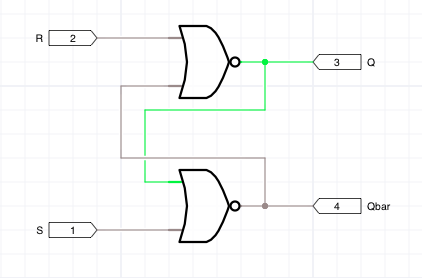
\includegraphics[width=0.5\textwidth]{./images/sr_diagram.png}
	\caption{\label{fig:sr_circuit_diagram}Circuit diagram of an S-R Latch using NOR gates.}
\end{center}
\end{figure}

\begin{table}[H]
\begin{center}
\begin{tabular}{| l | l | l | l | l |}
	\hline
	S & R & Q & Qbar & Comment \\ \hline
	0 & 0 & Q & Qbar & Hold \\ \hline
	0 & 1 & 0 & 1 & Reset \\ \hline
	1 & 0 & 1 & 0 & Set \\ \hline
	1 & 1 & 0 & 0 & Invalid Input \\ \hline
\end{tabular}
\caption{\label{tab:srTruthTable}Truth table for S-R Latch.}
\end{center}
\end{table}

\begin{table}[H]
\begin{center}
\begin{tabular}{| l | l | l |}
	\hline
	Bit & Label & Port \\ \hline
	S & Switch 1 & V16 \\ \hline
	R & Switch 0 & V17 \\ \hline
	clk & Clock & W5 \\ \hline
	Q & LED 0 & U16 \\ \hline
	Qbar & LED 1 & E19 \\ \hline
	error[0] & CA & W7 \\ \hline
	error[1] & CB & W6 \\ \hline
	error[2] & CC & U8 \\ \hline
	error[3] & CD & V8 \\ \hline
	error[4] & CE & U5 \\ \hline
	error[5] & CF & V5 \\ \hline
	error[6] & CG & U7 \\ \hline
\end{tabular}
\caption{\label{tab:srPorts}Port assignments for S-R Latch.}
\end{center}
\end{table}

\subsubsection{Results}
This design worked exactly as designed. All four possible input combinations are represented in Figures ~\ref{fig:srResultOne} through ~\ref{fig:srResultFour} below.

\begin{figure}[H]
\begin{center}
	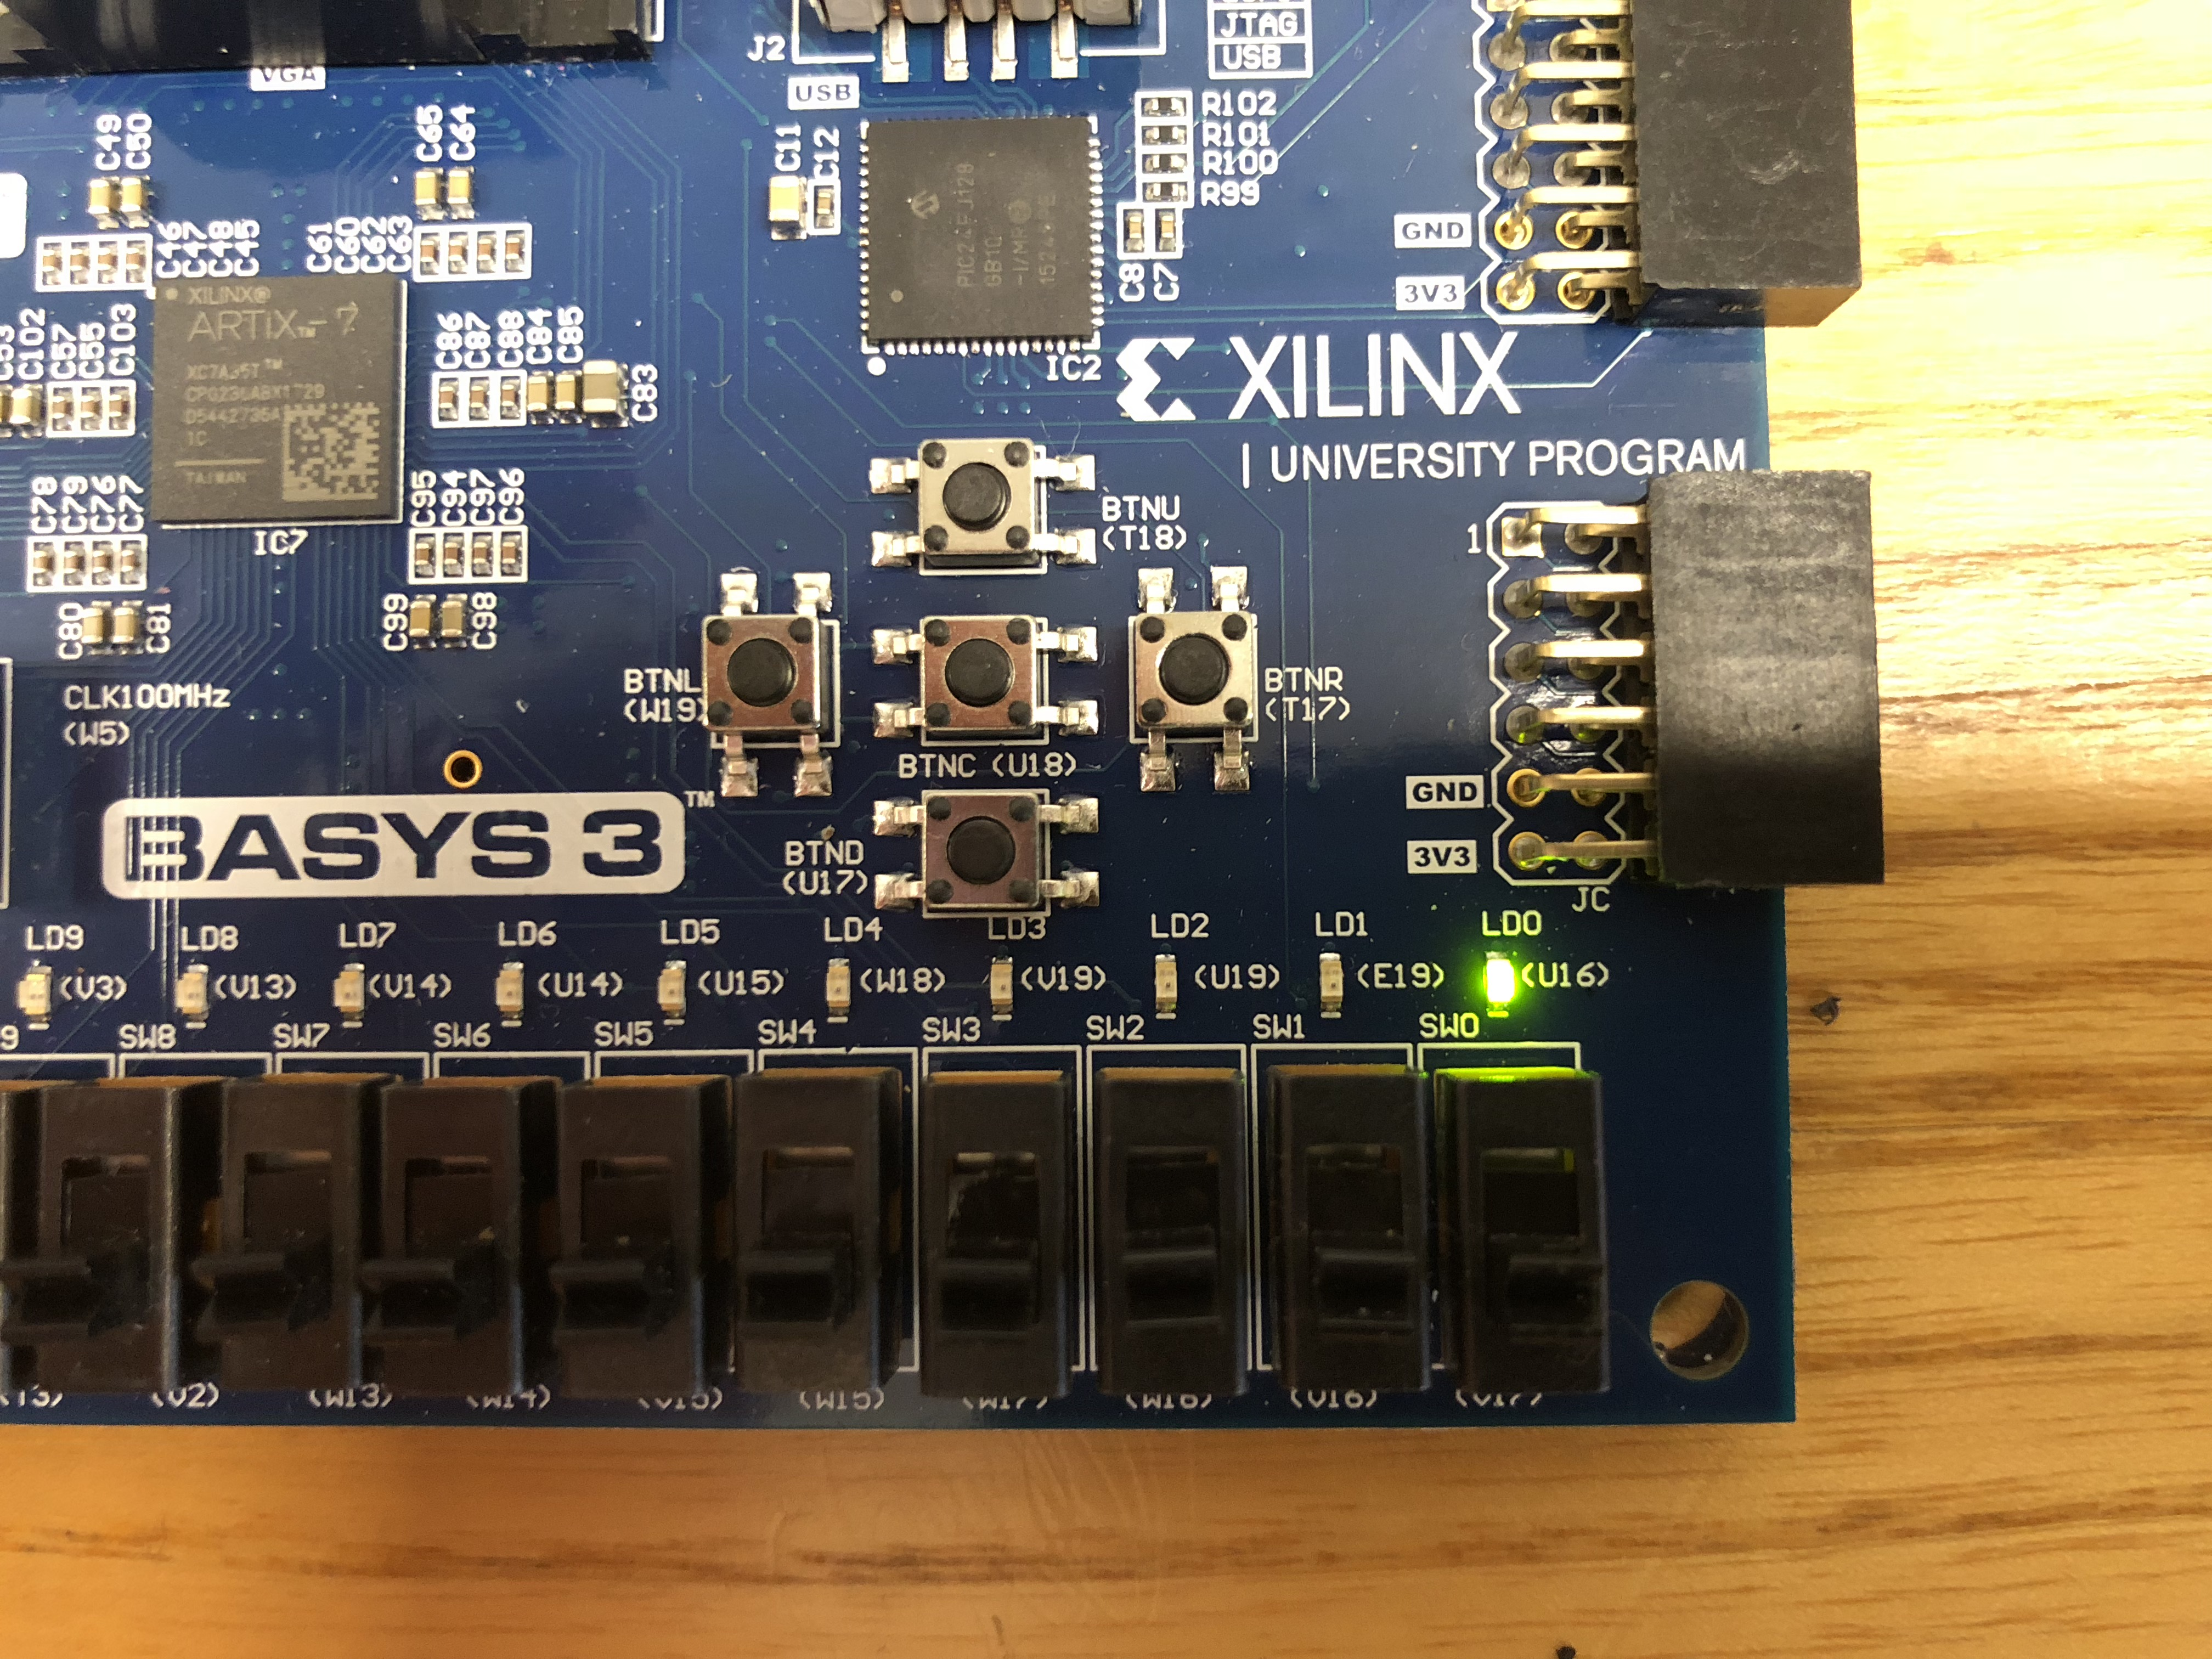
\includegraphics[width=0.5\textwidth]{./images/img_101.jpg}
	\caption{\label{fig:srResultOne}S-R inputs "00" result in a hold. Begin Q was on previously, it remains off now.}
\end{center}
\end{figure}

\begin{figure}[H]
\begin{center}
	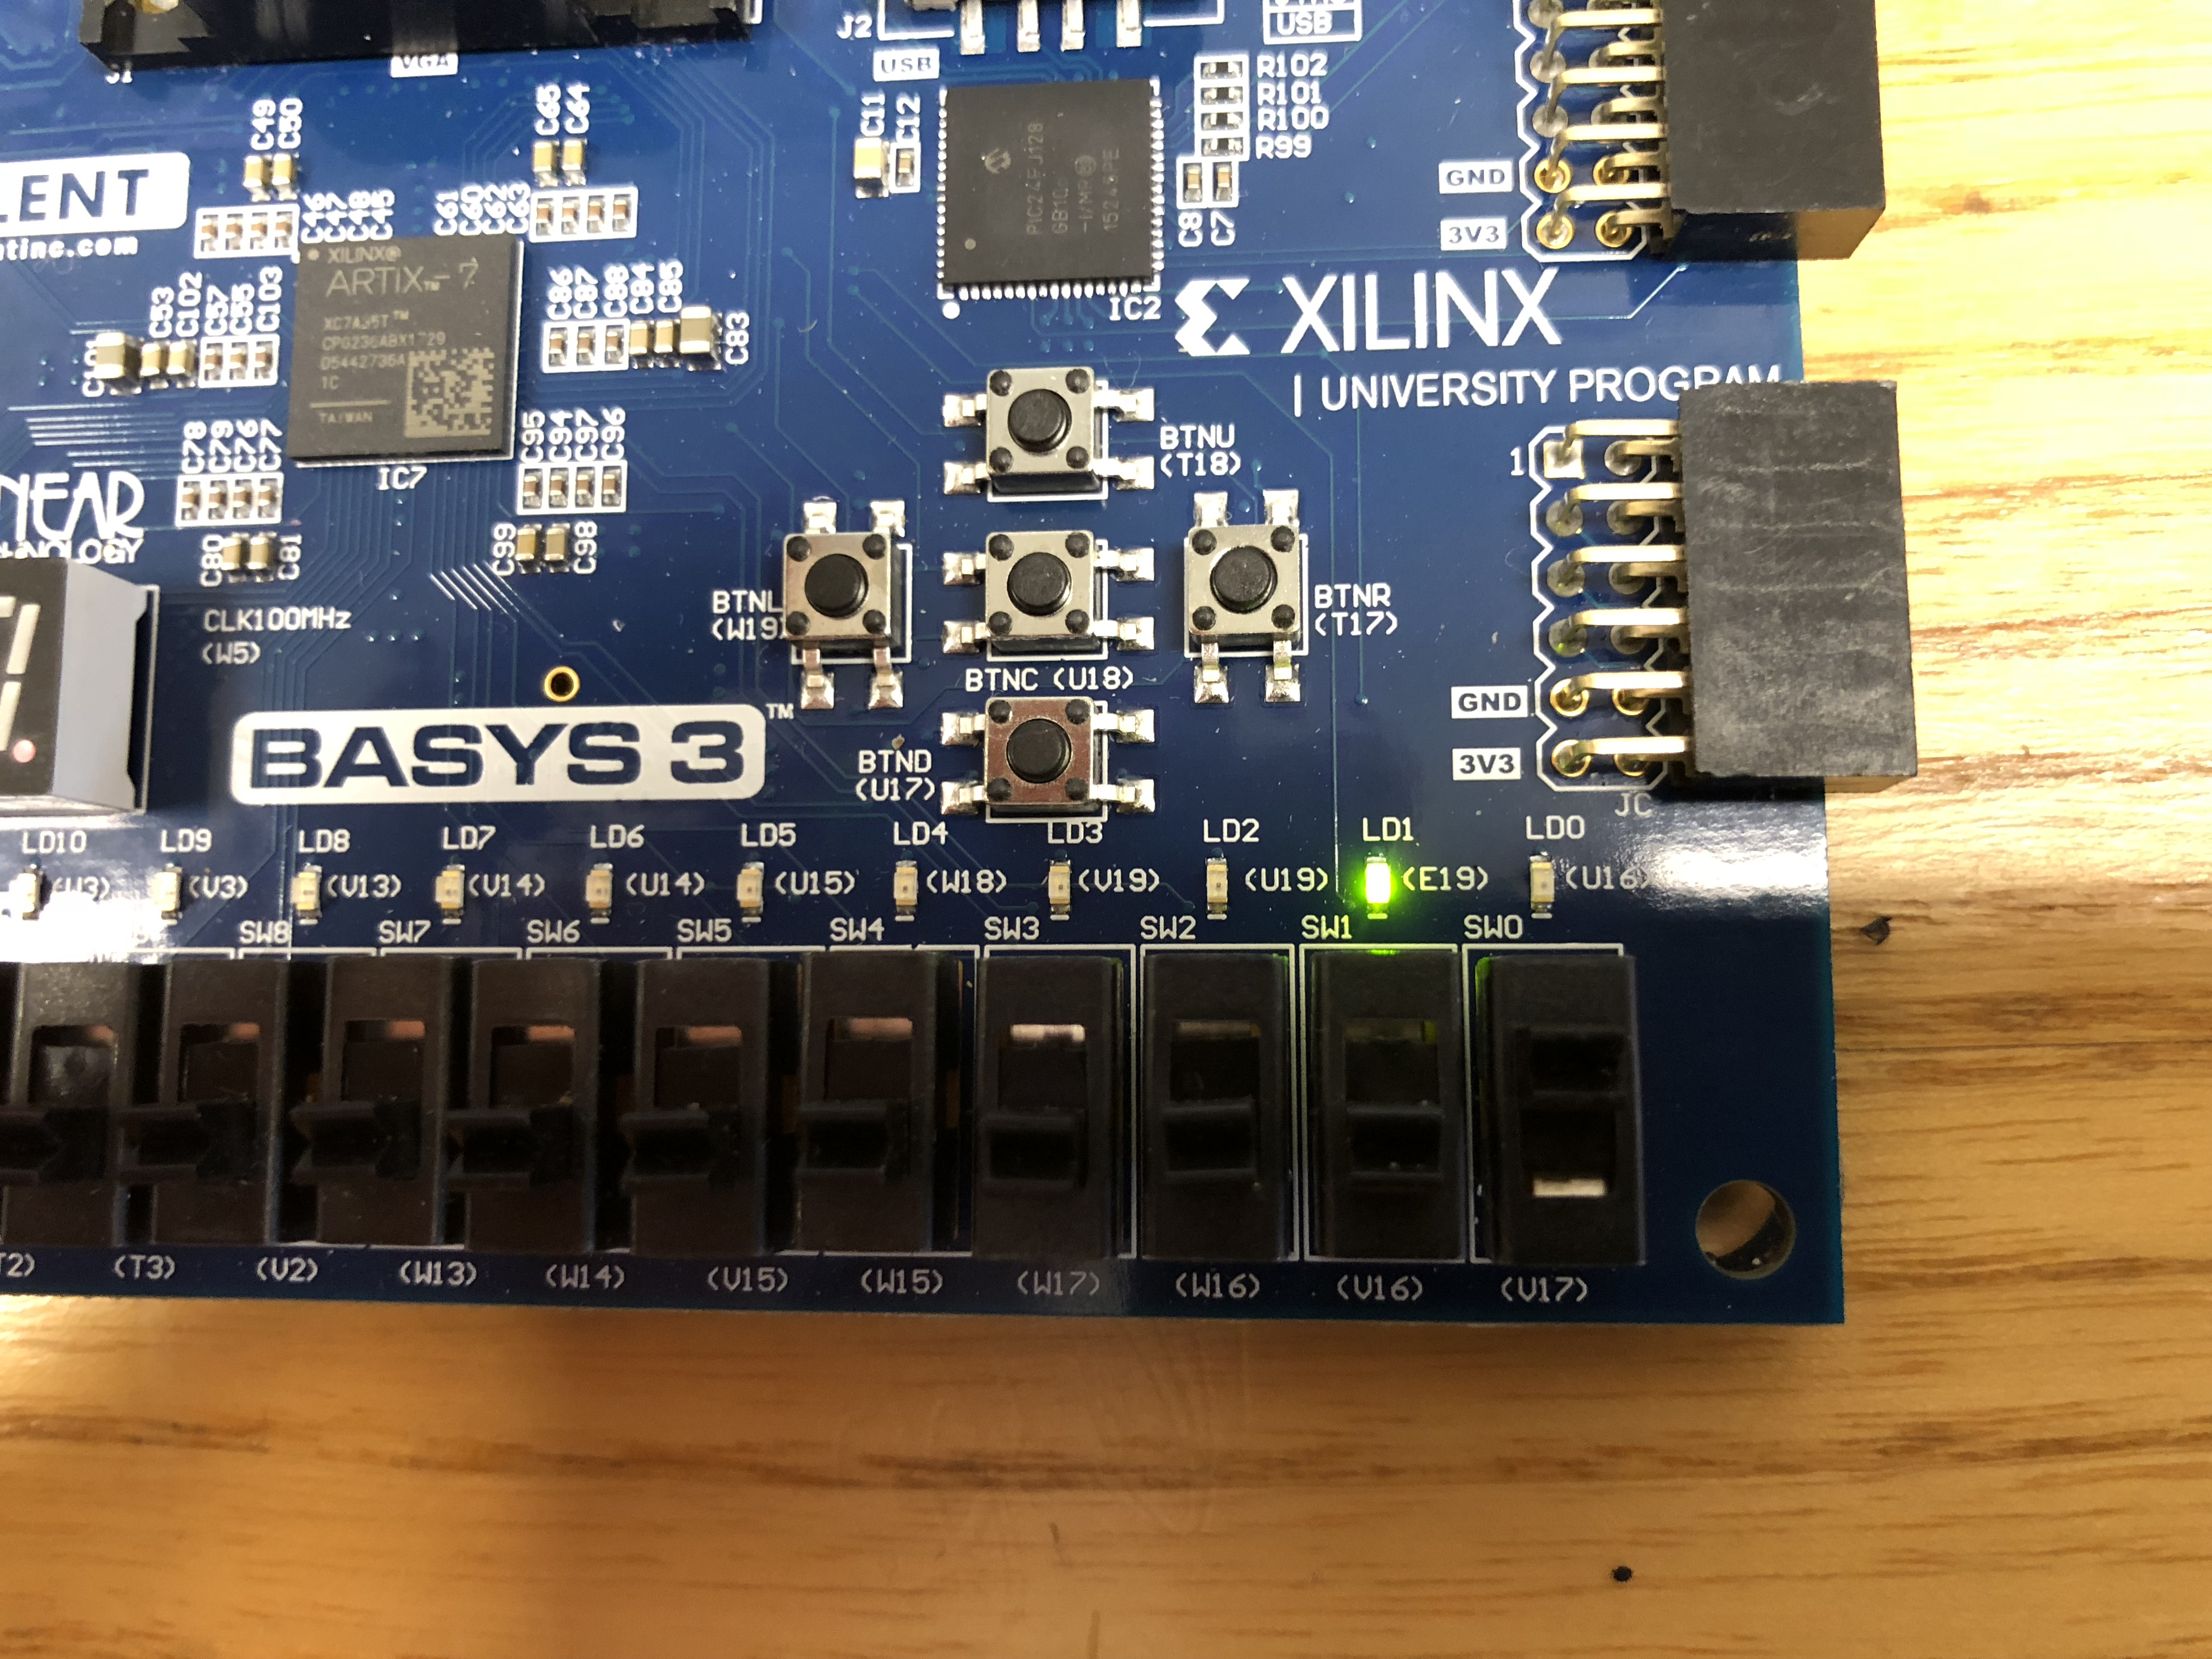
\includegraphics[width=0.5\textwidth]{./images/img_102.jpg}
	\caption{\label{fig:srResultTwo}S-R inputs "01" result in a reset, so Q goes off and Qbar goes on.}
\end{center}
\end{figure}

\begin{figure}[H]
\begin{center}
	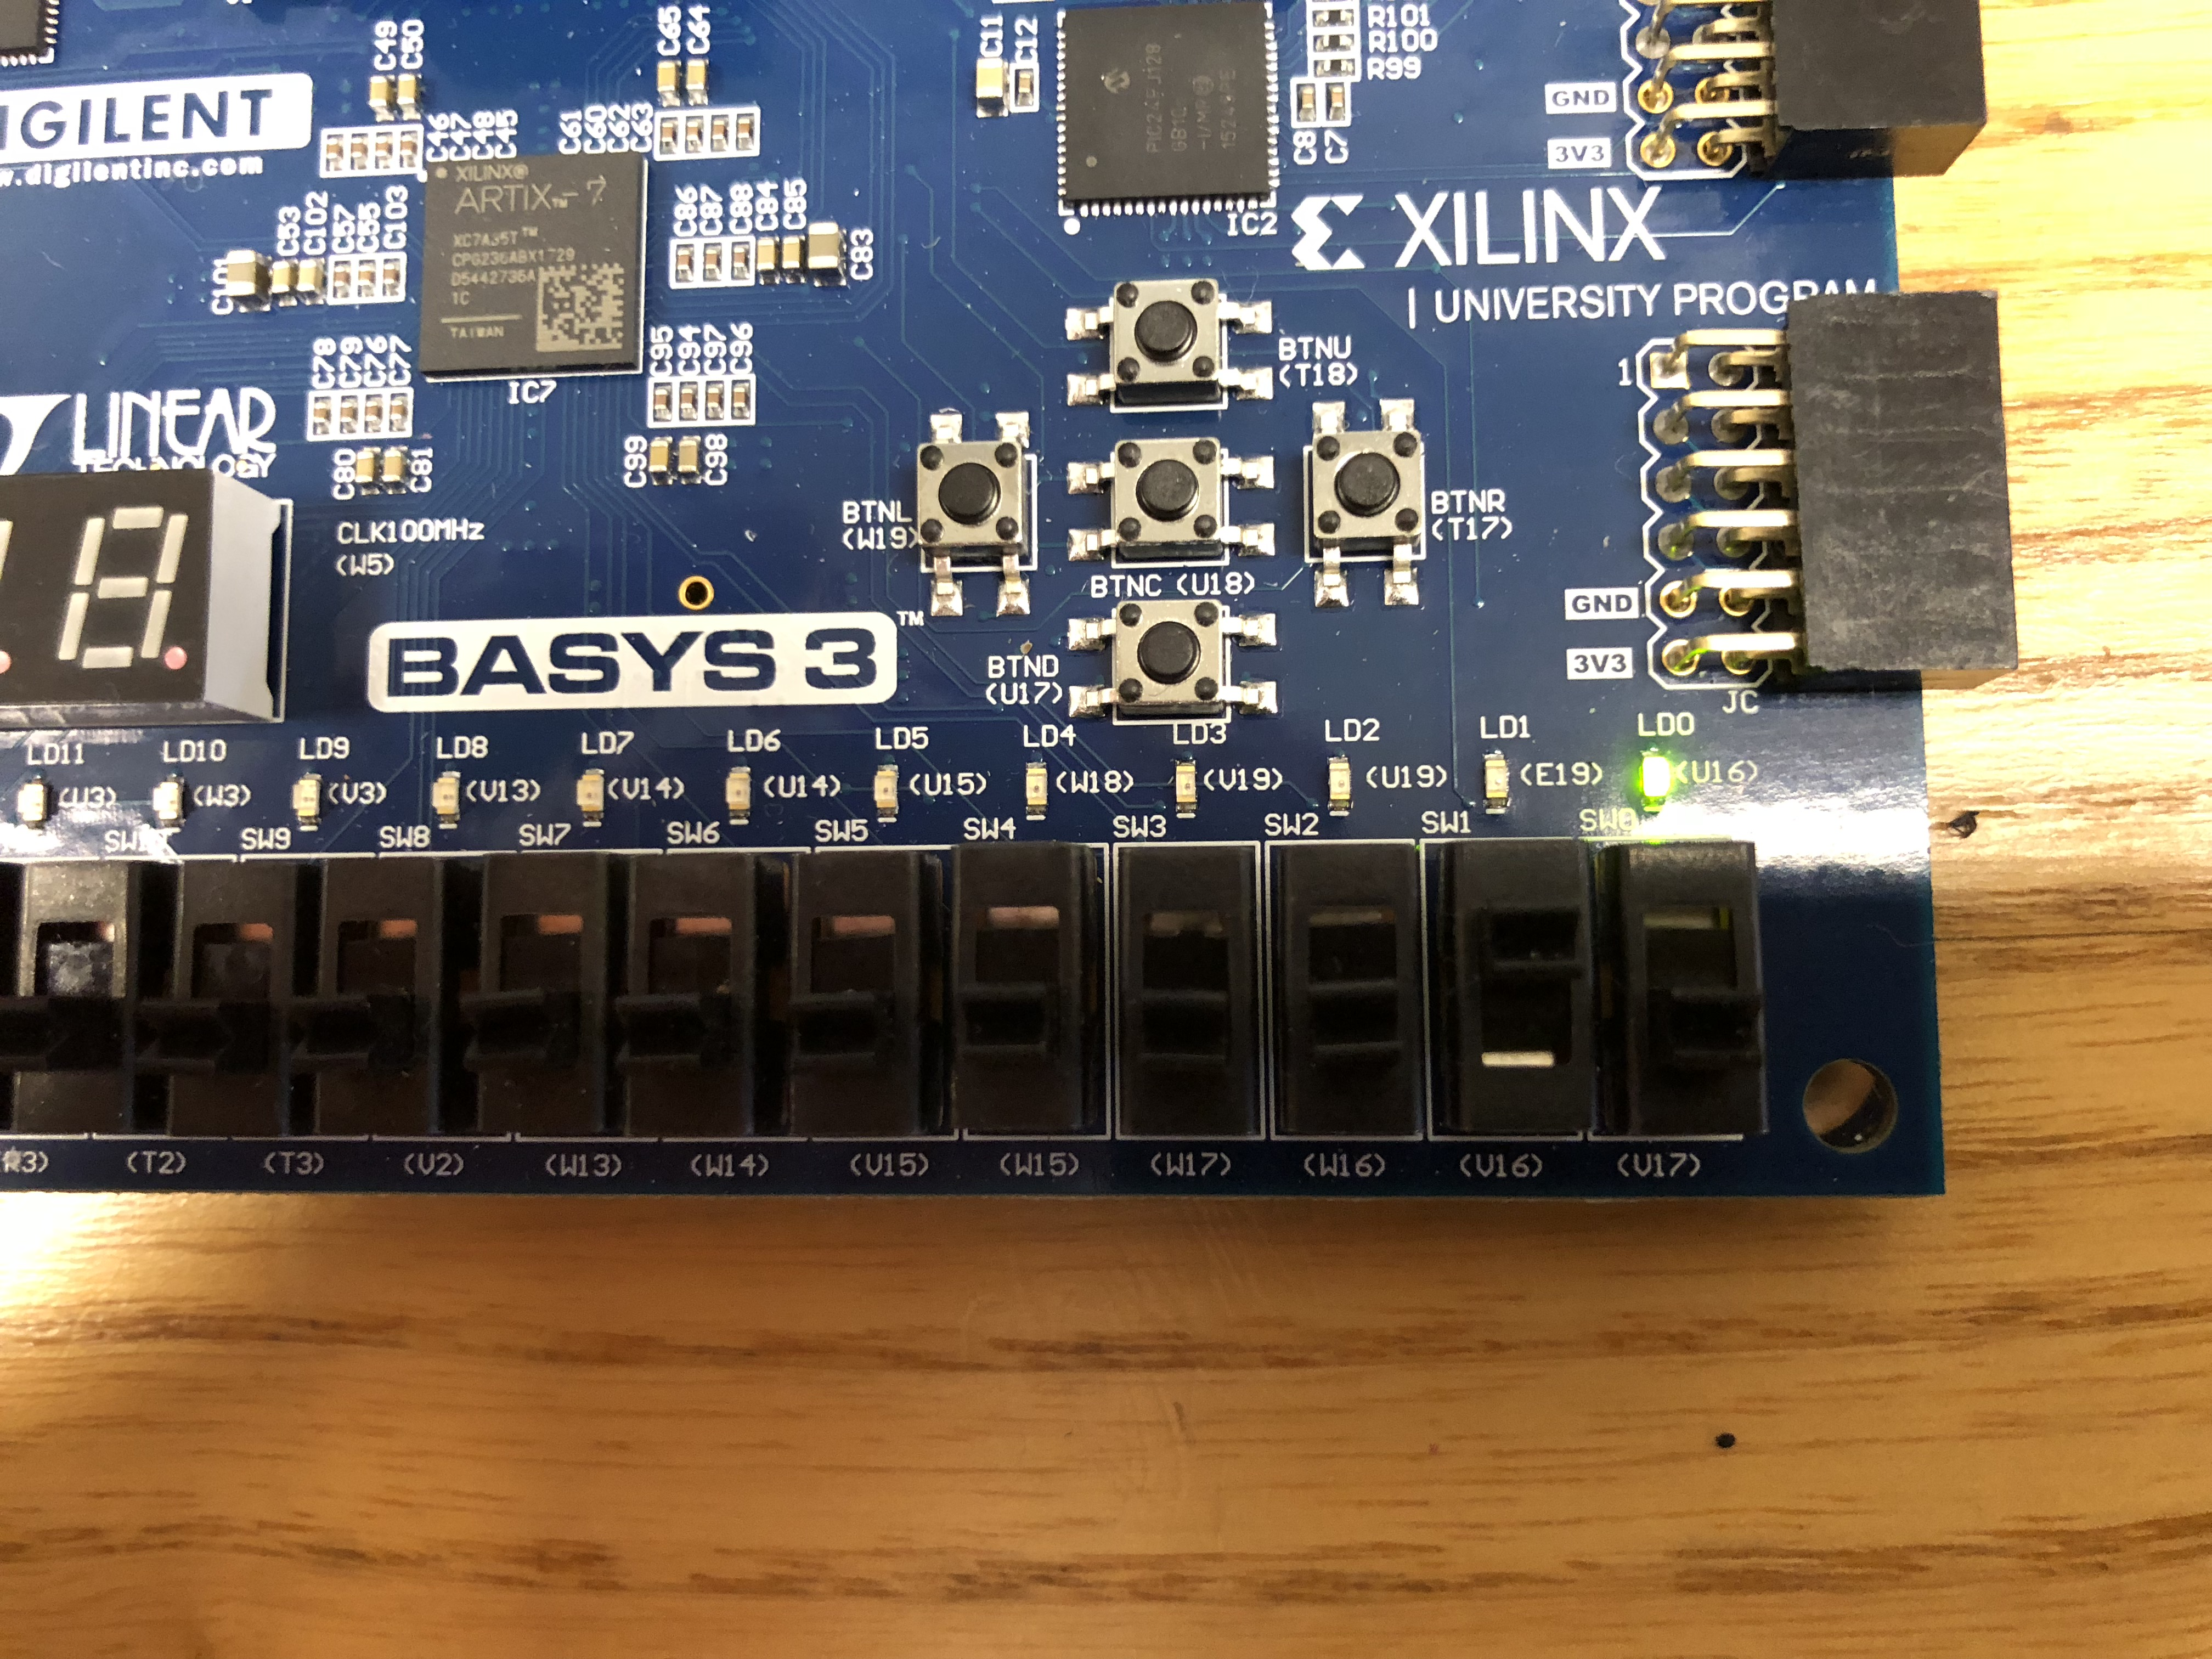
\includegraphics[width=0.5\textwidth]{./images/img_103.jpg}
	\caption{\label{fig:srResultThree}S-R inputs "10" result in a set. Therefore, Q goes back on, and Qbar goes off.}
\end{center}
\end{figure}

\begin{figure}[H]
\begin{center}
	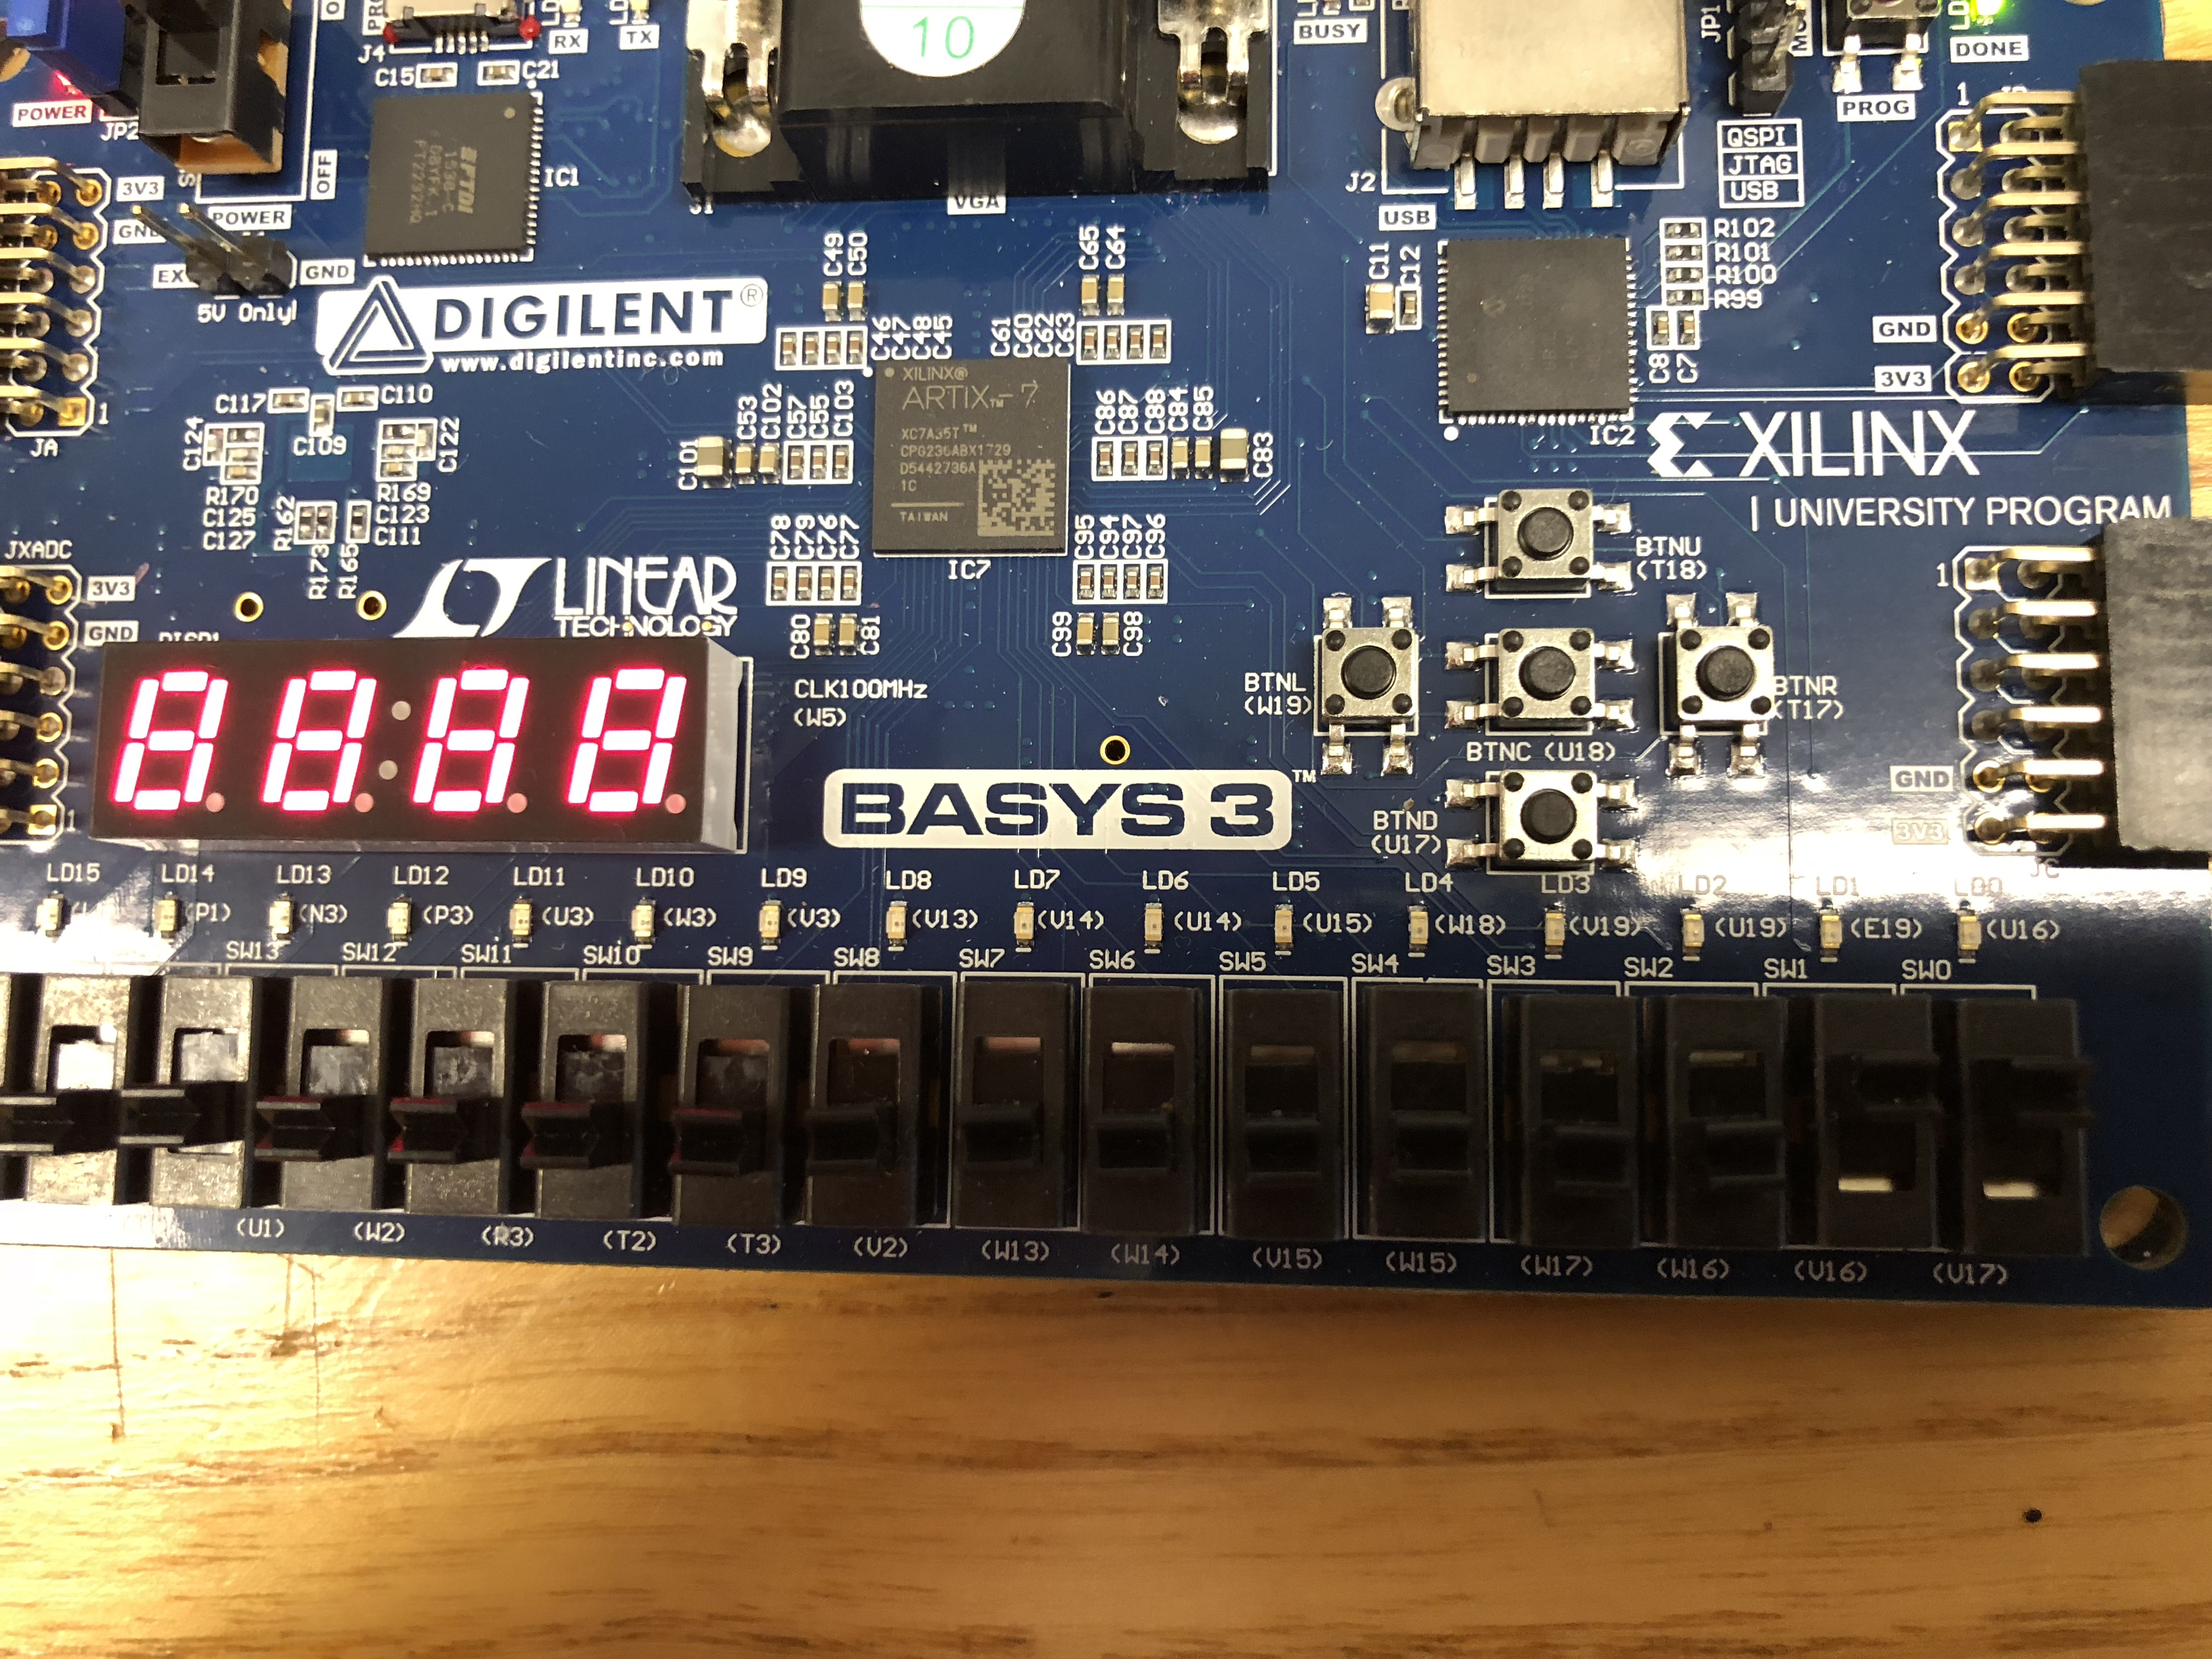
\includegraphics[width=0.5\textwidth]{./images/img_104.jpg}
	\caption{\label{fig:srResultFour}S-R inputs "11" result in an error state, so all LEDs go off and the 7-segment displays signal the error.}
\end{center}
\end{figure}

\subsection{Problem 2 }

\subsubsection{Background}
Problem 2 is to implement a D latch, by simply tying the single input to S and to R, using an inverter for one of them. The inverter will toggle the SR inputs from set to reset as it changes. Most of the code for this will be contained in a component of the S-R latch from Problem 1.

\subsubsection{Design Solution}
Because of the nature of this design, shown in Figure ~\ref{fig:d_circuit_diagram}, it is now impossible for the invalid state of "11" to be passed to the SR latch. Therefore, we tied the 'error' vector to a signal instead of worrying about an output assignment. This results in the truth table, Table ~\ref{tab:dTruthTable}. Port assignments for this design are summarized in ~\ref{tab:dPorts}.

\begin{figure}[H]
\begin{center}
	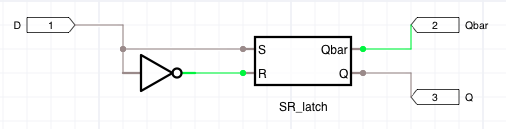
\includegraphics[width=0.5\textwidth]{./images/d_diagram.png}
	\caption{\label{fig:d_circuit_diagram}The circuit diagram for the D-latch incorporating an SR-latch.}
\end{center}
\end{figure}

\begin{table}[H]
\begin{center}
\begin{tabular}{| l | l | l |}
	\hline
	D & Q & Qbar \\ \hline
	0 & 0 & 1 \\ \hline
	1 & 1 & 0 \\ \hline
\end{tabular}
\caption{\label{tab:dTruthTable}Truth table for the D latch.}
\end{center}
\end{table}

\begin{table}[H]
\begin{center}
\begin{tabular}{| l | l | l |}
	\hline
	Bit & Label & Port \\ \hline
	D & Switch 0 & V17 \\ \hline
	clk & Clock & W5 \\ \hline
	Q & LED 0 & U16 \\ \hline
	Qbar & LED 1 & E19 \\ \hline
\end{tabular}
\caption{\label{tab:dPorts}Port assignments for the D latch.}
\end{center}
\end{table}

\subsubsection{Results}
There are only two possible states for this D latch, set or reset. We were able to implement and demonstrate each. The results are displayed in Figures ~\ref{fig:dResultOne} and ~\ref{fig:dResultTwo}.

\begin{figure}[H]
\begin{center}
	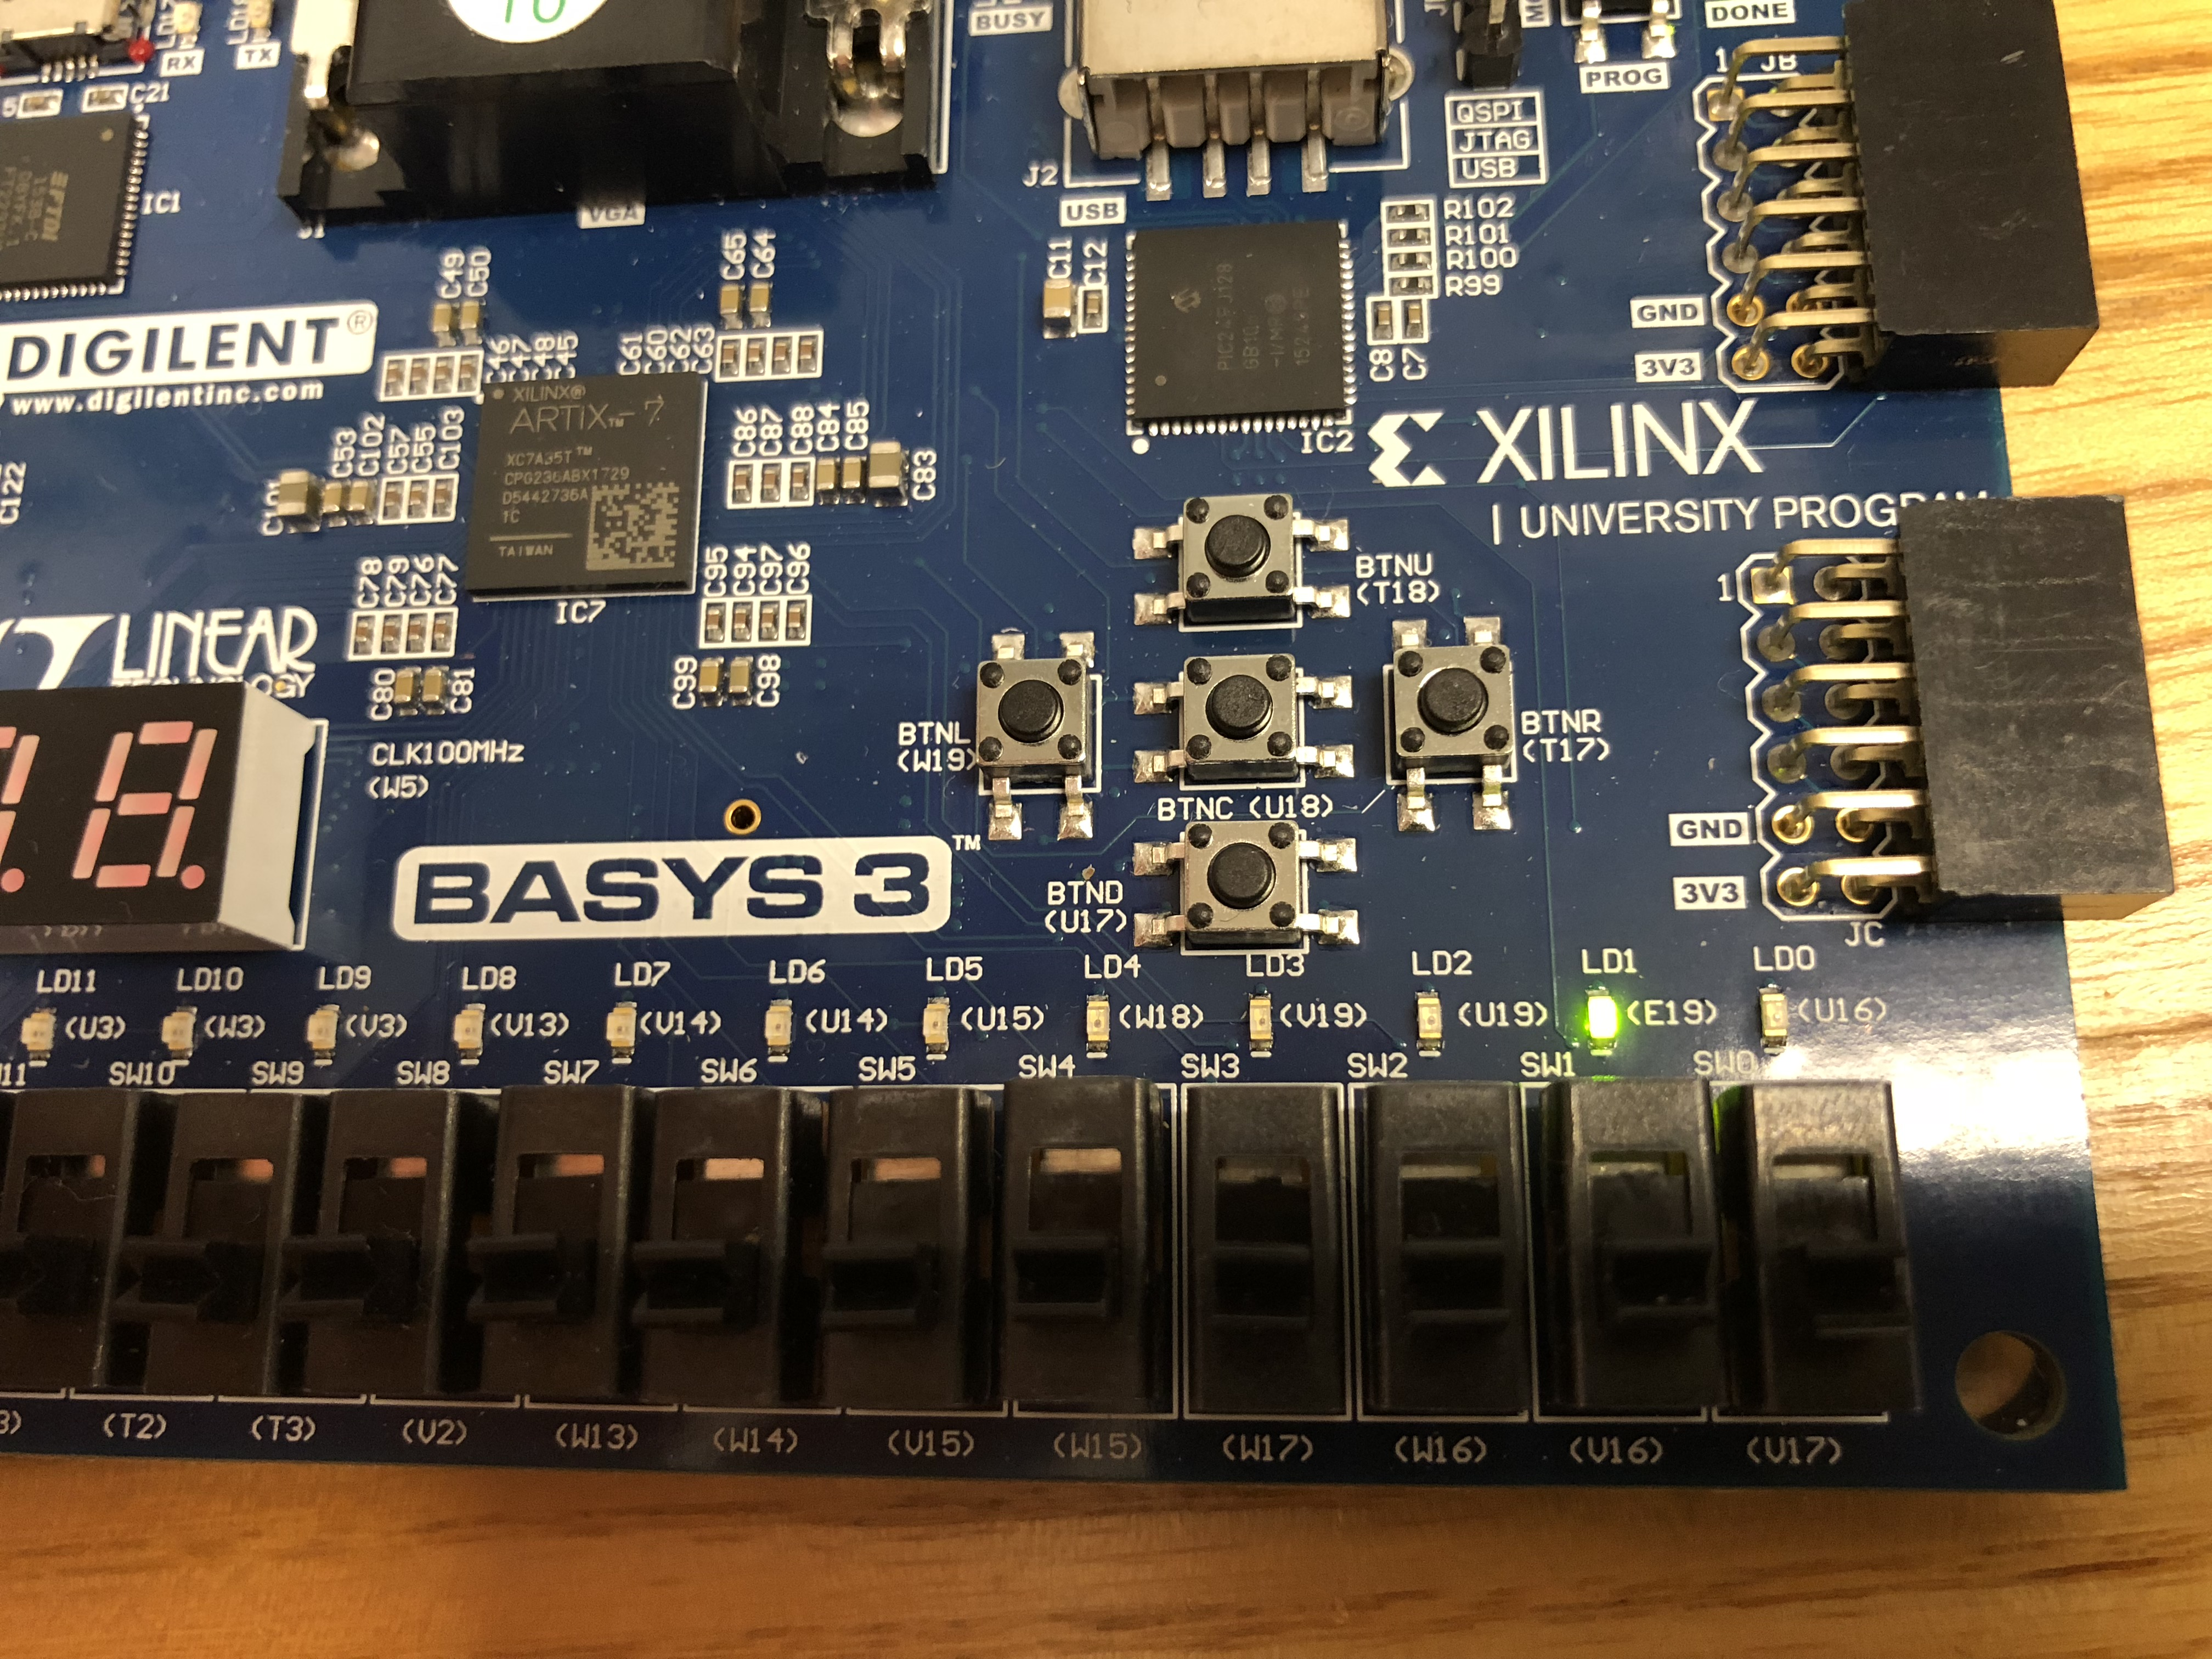
\includegraphics[width=0.5\textwidth]{./images/img_201.jpg}
	\caption{\label{fig:dResultOne}D is off, which results in a "reset" input. Therefore, Q is LOW or '0' and Qbar is HIGH or '1'.}
\end{center}
\end{figure}

\begin{figure}[H]
\begin{center}
	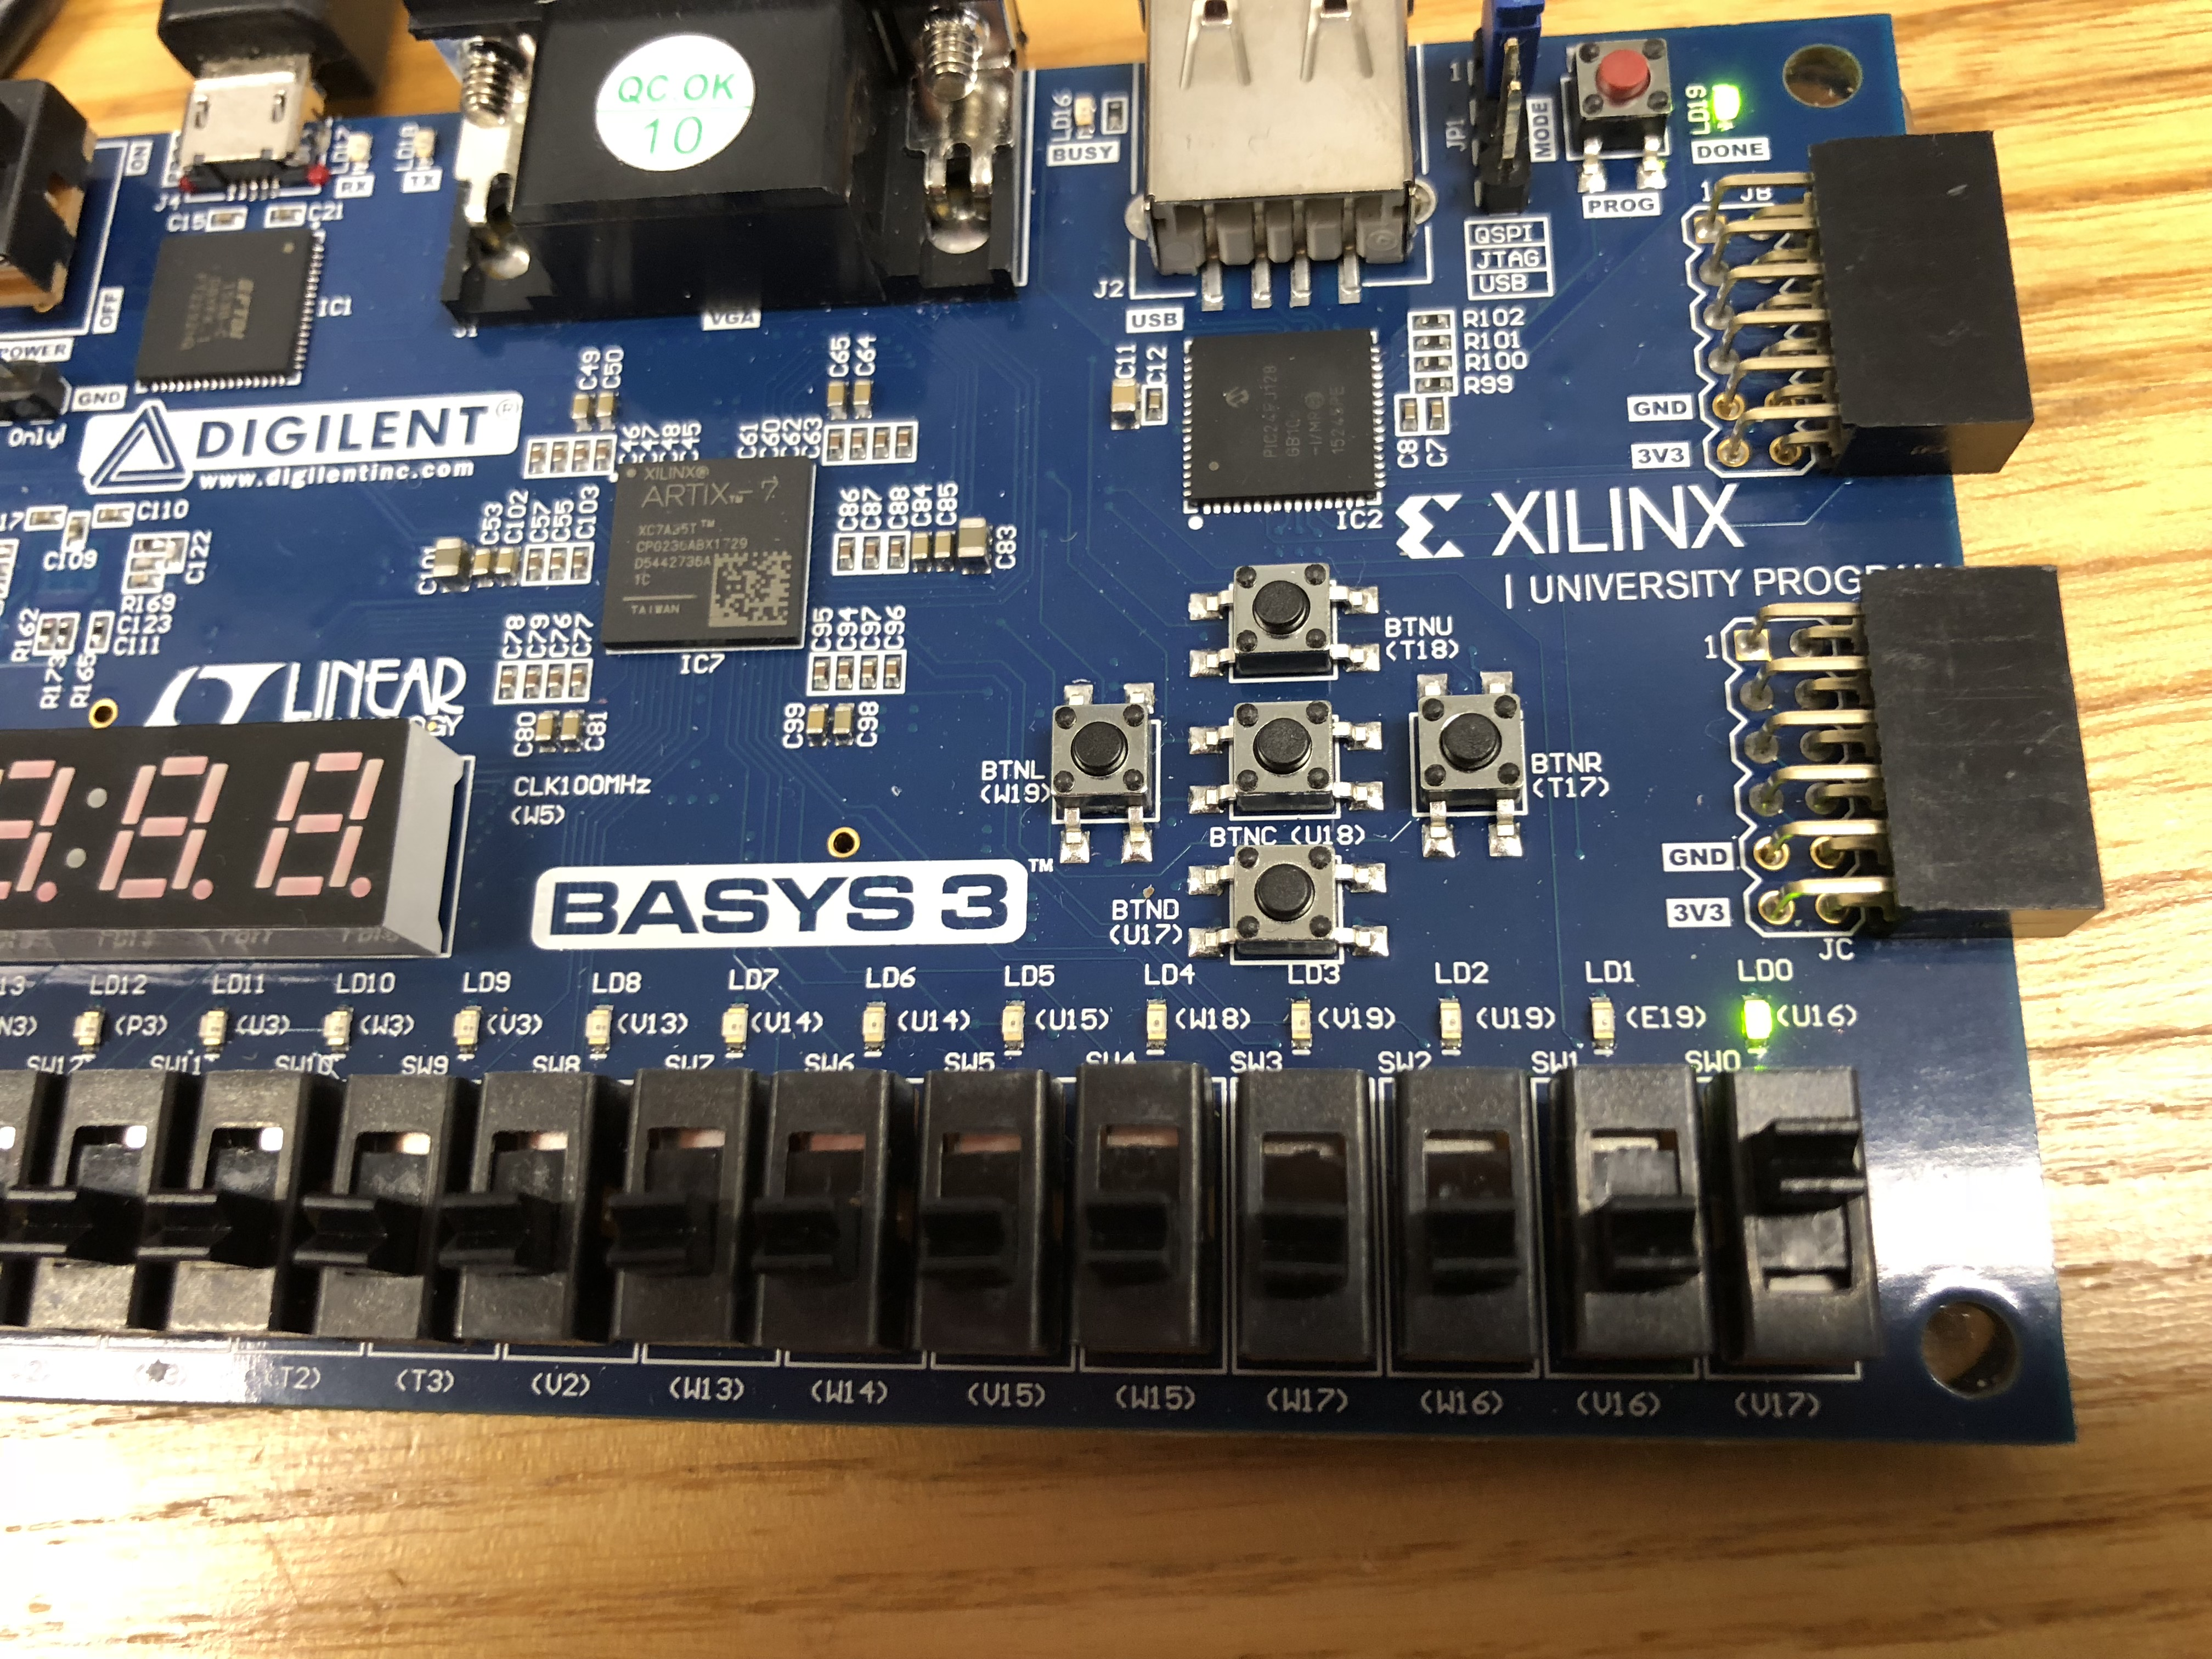
\includegraphics[width=0.5\textwidth]{./images/img_202.jpg}
	\caption{\label{fig:dResultTwo}D is on, which results in a "set" input. Therefore, Q is HIGH or '1' and Qbar is LOW or '0'.}
\end{center}
\end{figure}

\subsection{Problem 3}

\subsubsection{Background}
Problem 3 adds an "enable" and an asynchronous "reset" to the S-R latch from Problem 1. The SR latch will only be activated when "enable" is '1' or HIGH. Additionally, regardless of the clock state, the output will immediately go to '0' or LOW when "reset" is HIGH or '1'.

\subsubsection{Design Solution}
We implemented the enable bit by tying the S and R inputs to AND gates with "enable" as shown in Figure ~\ref{fig:modifiedSR_circuit_diagram}. However, we were unable to implement an asynchronous reset.

\begin{figure}[H]
\begin{center}
	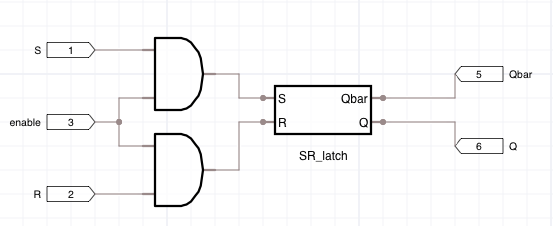
\includegraphics[width=0.5\textwidth]{./images/sr_diagram2.png}
	\caption{\label{fig:modifiedSR_circuit_diagram}The modified S-R Latch circuit that includes an enable.}
\end{center}
\end{figure}

\begin{table}[H]
\begin{center}
\begin{tabular}{| l | l | l | l | l | l |}
	\hline
	S & R & Enable & Reset & Q & Qbar \\ \hline
	- & - & - & 1 & 0 & 1 \\ \hline
	0 & 0 & 1 & 0 & Q & Qbar \\ \hline
	0 & 1 & 1 & 0 & 0 & 1  \\ \hline
	1 & 0 & 1 & 0 & 1 & 0 \\ \hline
	1 & 1  & 1 & 0 & err & err \\ \hline
	0 & 0 & 0 & 0 & Q & Qbar \\ \hline
	0 & 1 & 0 & 0 & Q & Qbar \\ \hline
	1 & 0 & 0 & 0 & Q & Qbar \\ \hline
	1 & 1 & 0 & 0 & Q & Qbar \\ \hline
\end{tabular}
\end{center}
\end{table}

\subsubsection{Results}
We were not able to achieve a functioning solution for this problem.

\section{Conclusion}
The most difficult technical challenge in this lab related directly to the use of synchronous and asynchronous items together with components. We were unable to accomplish problem 3 because of the difficulty of integrating a synchronous component that could be overridden from outside the component. However, we did gain a greater working understanding of latches, and especially of synchronous operations from this lab.

\pagebreak

\textbf{Appendices}

\begin{appendices}

\section{Problem 1 VHDL Code}

\begin{lstlisting}[language=VHDL]
library IEEE;
use IEEE.STD_LOGIC_1164.ALL;

-- Declares an SR latch, which will be able to set, reset, and store memory
entity sr_latch is
    Port ( s : in STD_LOGIC;
           r : in STD_LOGIC;
           clk : in STD_LOGIC;
           q : inout STD_LOGIC;
           qbar : inout STD_LOGIC;
           error : out STD_LOGIC_VECTOR(6 downto 0));
end sr_latch;

architecture sr_arch of sr_latch is

begin
	-- latches are synchronous, so we are inside a clock process
    process(clk)
    begin
    		-- if on a rising clock edge, then we act
        if(clk'event and (clk='1')) then
        	-- this ia an invalid state
            if((r = '1') and (s = '1')) then
                q <= '0';
                qbar <= '0';
                -- turns on the 7-segment display
                error <= "0000000";
            else
                q <= r nor qbar;
                qbar <= s nor q;
                error <= "1111111";
            end if;
        end if;
    end process;
end sr_arch;
\end{lstlisting}

\section{Problem 1 Constraints File}
\begin{figure}[H]
\begin{center}
	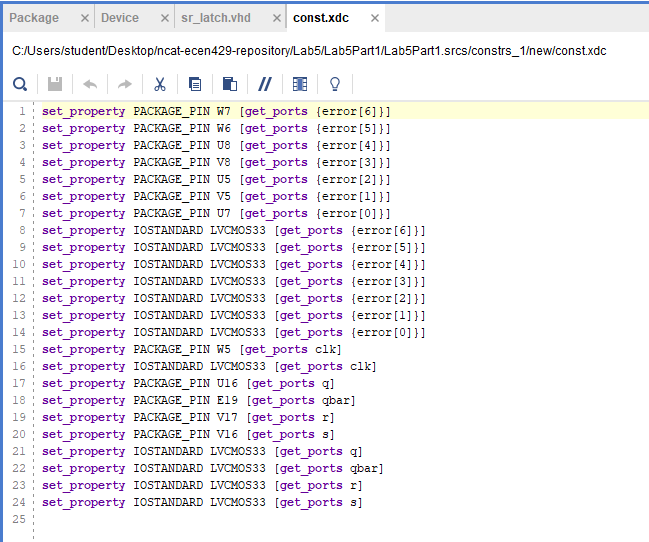
\includegraphics[width=0.5\textwidth]{./images/Lab5Part1Const.png}
	\caption{\label{fig:Part1ConstFile}Constraints file for Problem 1.}
\end{center}
\end{figure}

\section{Problem 2 VHDL Code}
\begin{lstlisting}[language=VHDL]
library IEEE;
use IEEE.STD_LOGIC_1164.ALL;

-- Declares an SR latch, which will be able to set, reset, and store memory
entity sr_latch is
    Port ( s : in STD_LOGIC;
           r : in STD_LOGIC;
           clk : in STD_LOGIC;
           q : inout STD_LOGIC;
           qbar : inout STD_LOGIC;
           error : out STD_LOGIC_VECTOR(6 downto 0));
end sr_latch;

architecture sr_arch of sr_latch is

begin
	-- latches are synchronous, so we are inside a clock process
    process(clk)
    begin
    		-- if on a rising clock edge, then we act
        if(clk'event and (clk='1')) then
        	-- this ia an invalid state
            if((r = '1') and (s = '1')) then
                q <= '0';
                qbar <= '0';
                -- turns on the 7-segment display
                error <= "0000000";
            else
                q <= r nor qbar;
                qbar <= s nor q;
                error <= "1111111";
            end if;
        end if;
    end process;
end sr_arch;
library IEEE;
use IEEE.STD_LOGIC_1164.ALL;

entity d_flipflop is
    Port ( d : in STD_LOGIC;
           clk : in STD_LOGIC;
           q : inout STD_LOGIC;
           qbar : inout STD_LOGIC);
end d_flipflop;

architecture d_arch of d_flipflop is

component sr_latch is port( s : in STD_LOGIC;
           r : in STD_LOGIC;
           clk : in STD_LOGIC;
           q : inout STD_LOGIC;
           qbar : inout STD_LOGIC;
           error : out STD_LOGIC_VECTOR(6 downto 0));
end component sr_latch;

signal error_sig : STD_LOGIC_VECTOR(6 downto 0);
signal dbar : STD_LOGIC;

begin
	--this component instantiation ties d to S and dbar to R
    sr_comp : sr_latch port map(d, dbar, clk, q, qbar, error_sig);
    
    process(clk)
    begin
        if(clk'event and (clk='1')) then
        		--this part simplies ties dbar to an inverted d
            dbar <= not d;
        end if;
    end process;
end d_arch;
\end{lstlisting}

\section{Problem 2 Constraints File}
\begin{figure}[H]
\begin{center}
	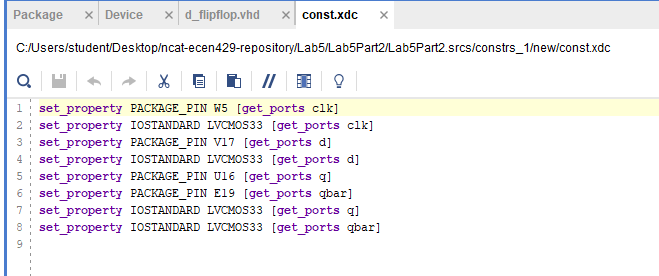
\includegraphics[width=0.5\textwidth]{./images/Lab5Part2Const.png}
	\caption{\label{fig:Part2ConstFile}Constraints file for Problem 2.}
\end{center}
\end{figure}

\section{Problem 3 VHDL Code}
\begin{lstlisting}[language=VHDL]
library IEEE;
use IEEE.STD_LOGIC_1164.ALL;

-- Declares an SR latch, which will be able to set, reset, and store memory
entity sr_latch is
    Port ( s : in STD_LOGIC;
           r : in STD_LOGIC;
           clk : in STD_LOGIC;
           q : inout STD_LOGIC;
           qbar : inout STD_LOGIC;
           error : out STD_LOGIC_VECTOR(6 downto 0));
end sr_latch;

architecture sr_arch of sr_latch is

begin
	-- latches are synchronous, so we are inside a clock process
    process(clk)
    begin
    		-- if on a rising clock edge, then we act
        if(clk'event and (clk='1')) then
        	-- this ia an invalid state
            if((r = '1') and (s = '1')) then
                q <= '0';
                qbar <= '0';
                -- turns on the 7-segment display
                error <= "0000000";
            else
                q <= r nor qbar;
                qbar <= s nor q;
                error <= "1111111";
            end if;
        end if;
    end process;
end sr_arch;

library IEEE;
use IEEE.STD_LOGIC_1164.ALL;

entity sr_latch_reset is
    Port ( s : in STD_LOGIC;
           r : in STD_LOGIC;
           clk : in STD_LOGIC;
           reset : in STD_LOGIC;
           enable : in STD_LOGIC;
           q : inout STD_LOGIC;
           qbar : inout STD_LOGIC);
end sr_latch_reset;

architecture sr_reset_arch of sr_latch_reset is

component sr_latch is port( s : in STD_LOGIC;
           r : in STD_LOGIC;
           clk : in STD_LOGIC;
           q : inout STD_LOGIC;
           qbar : inout STD_LOGIC;
           error : out STD_LOGIC_VECTOR(6 downto 0));
end component sr_latch;

signal error_sig : STD_LOGIC_VECTOR(6 downto 0);

begin
    sr_comp : sr_latch port map(s, r, clk, q, qbar, error_sig);
    
    process(reset, clk)
    begin
        if(reset = '1') then
            q <= '0';
            qbar <= '1';
        elsif(clk'event and (clk = '1') and enable = '0') then
            q <= '0';
            qbar <= '1';
        end if;
    end process;

end sr_reset_arch;
\end{lstlisting}

\section{Problem 3 Constraints File}
\begin{figure}[H]
\begin{center}
	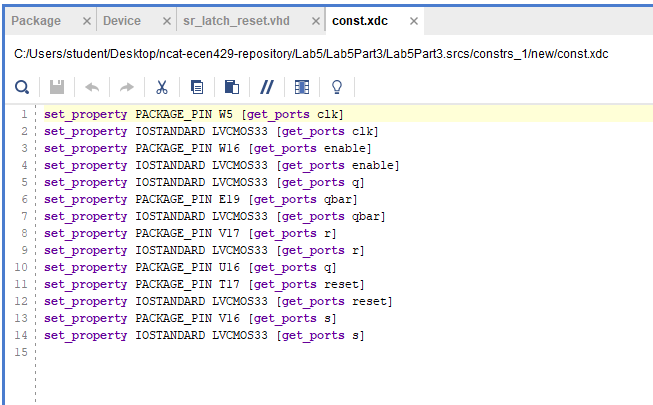
\includegraphics[width=0.5\textwidth]{./images/Lab5Part3Const.png}
	\caption{\label{fig:Part3ConstFile}Constraints file for Problem 3.}
\end{center}
\end{figure}

\end{appendices}
\end{document}
